\documentclass[16pt]{beamer}
\usepackage[utf8]{inputenc}
\usepackage[croatian]{babel}
\usepackage{graphicx}
\usepackage{graphicx}
\usepackage{verbatim}
\usepackage{bookmark}
\usepackage{pgfplots}

\graphicspath{ {figures/} }
\usepackage{array}
\usetheme{Warsaw}
\definecolor{mygreen}{rgb}{0.3, 0.73, 0.09}
\setbeamercolor*{palette primary}{use=structure,fg=black,bg=mygreen}
\definecolor{mygreen1}{rgb}{0.0, 0.5, 0.0}
\setbeamercolor*{palette quaternary}{fg=black,bg=mygreen1}
\newcommand\Fontvi{\fontsize{6,5}{7.5}\selectfont}
\newcommand\Fon{\fontsize{8}{7.5}\selectfont}

\pgfplotsset{width=10cm,height=8cm}


\pgfplotsset{every axis/.append style={
                    axis x line=middle,    
                    axis y line=middle,    
                    axis line style={<->,color=blue}, 
                    xlabel={$x$},          
                    ylabel={$y$},          
            }}

\title[IZRADA TABLICA I GRAFIKONA\hspace{20mm} \insertframenumber/\inserttotalframenumber]{IZRADA TABLICA I GRAFIKONA}
\author{Anamaria Vargić \  Jelena Stojković  \  Valentina Ecimović}
\institute{Tehnički fakultet u Rijeci - Računarstvo}
\date{2018}
 
\begin{document}


\frame{\titlepage}
%slajd sa sadrzajem
\begin{frame}

\frametitle{Sadržaj}

\tableofcontents

\end{frame}
\begin{frame}
\frametitle{Lista tabela i slika}


\listoffigures
 
\listoftables
 
\newpage
 
\pagenumbering{arabic}
\end{frame} 

\begin{frame}

\frametitle{Izrada grafikona}

\begin{itemize}
\setlength\itemsep{1em}

\item za vizualiziranje podataka koristimo \textbf{pgfplots} package s kojime dobijemo autogenerirane grafikone

\item \textbf{pgfplots} package iz tikz/pgf omogućuje nam izradu grafikona iz podataka direktno iz .csv datoteka 
\item buduci da je \textbf{pgfplots} baziran na \textbf{tikz}-u grafikon se mora nalaziti unutar \textit{tikzpicture} okružja


\end{itemize}

\end{frame}



\begin{frame}[fragile]
\frametitle{Izrada grafikona}

\begin{itemize}
\setlength\itemsep{1em}

\item kako bi uključili \textbf{pgfplots} u dokument u preamblu moramo upisati:
	\begin{verbatim}
		\usepackage{pgfplots}
	\end{verbatim}
\item dodatne postavke za taj paket se mogu upisati u preamblu kao npr:
	\begin{verbatim}
		\pgfplotsset{width=2cm,compat=2.0}
	\end{verbatim}
	width mijenja veličinu svake pgfplot figure na 2 cm,compat određuje koju verziju paketa ćemo koristiti
		
	
\end{itemize}

\end{frame}

\begin{frame}

\frametitle{Izrada grafikona}

\begin{itemize}
\item korisnik mora unjeti samo podatke kao npr.
\begin{itemize}
\item oznake za osi koordinatnog sustava
\item unose za legende 
\item koordinate točaka
\end{itemize}

i \textbf{pgfplots} će na temelju tih podataka izraditi grafikon

\item izrađuje normalne, logaritamske i polulogaritamske grafikone u 2 ili 3 dimenzije 



\end{itemize}

\end{frame}

\begin{frame}[fragile]
\frametitle{Primjer jednostavnog grafikona}
\Fon
\begin{verbatim}

\documentclass{article}
\usepackage[margin=0.5in]{geometry}
\usepackage[utf8]{inputenc}

\usepackage{pgfplots}
\pgfplotsset{width=10cm,compat=1.9}

\begin{document}



\begin{tikzpicture}
\begin{axis}
\addplot[color=red]{exp(x)};
\end{axis}
\end{tikzpicture}



\end{document}

\end{verbatim}

\end{frame}


\begin{frame}[fragile]
\frametitle{Primjer jednostavnog grafikona}
\begin{tikzpicture}
\begin{axis}
\addplot[color=red]{exp(x)};
\end{axis}
\end{tikzpicture}
\end{frame}

\begin{frame}[fragile]

\frametitle{Parametarski grafikon - primjer}
\Fontvi

\begin{verbatim}
\documentclass{article}
\usepackage{pgfplots}
\pgfplotsset{width=15cm,height=15cm} %dimenzije grafa

\pgfplotsset{every axis/.append style={
                    axis x line=middle,    % pozicionira x os u sredinu
                    axis y line=middle,    % pozicionira y os u sredinu
                    axis line style={<->,color=blue}, % stavlja strelice na osi
                    xlabel={$x$},          % označava x-os sa oznakom x
                    ylabel={$y$},          % označava y-os sa oznakom y
            }}

\begin{document}

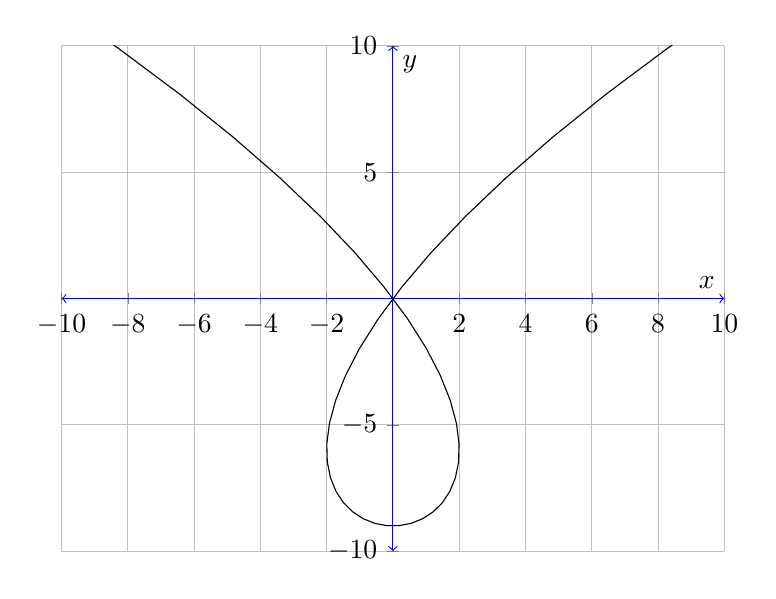
\begin{tikzpicture}  % tikzpicture okružje
    \begin{axis}[
            xmin=-10,xmax=10, % određuje granice x-osi
            ymin=-10,ymax=10, % određuje granice y-osi
            grid=both,
            ]
            \addplot [domain=-3:3,samples=50]({x^3-3*x},{3*x^2-9}); 
    \end{axis}
\end{tikzpicture}
\end{document}
\end{verbatim}



\end{frame}

\begin{frame}[fragile]
\frametitle{Parametarski grafikon - primjer}

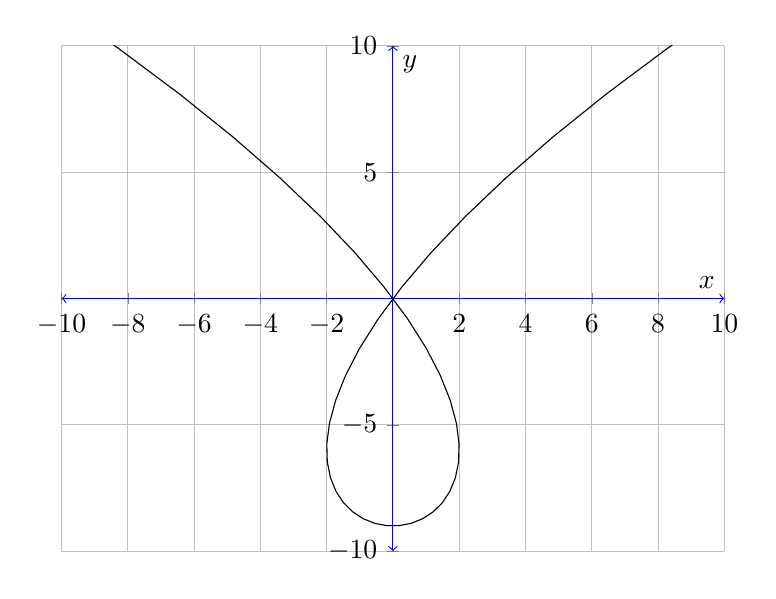
\begin{tikzpicture}
    \begin{axis}[
            xmin=-10,xmax=10,
            ymin=-10,ymax=10,
            grid=both,
            ]
            \addplot [domain=-3:3,samples=50]({x^3-3*x},{3*x^2-9}); 
    \end{axis}
\end{tikzpicture}
\end{frame}
%jelena
\begin{frame}[fragile]
\frametitle{2D grafikoni}

\textbf{2D} grafikone možete persionalizirati tj. prilagoditi ih svojim potrebama.
Oni mogu predstavljati npr: 
\begin{itemize}
\item matematički dijagram 

\item temperaturni dijagram 

\item podatkovani dijagram itd. 

\end{itemize}


\end{frame}
%kod matematicki
\begin{frame}[fragile]
\frametitle{Primjer matematičkog grafikona}
\Fontvi
\begin{verbatim}
\documentclass[10pt]{article}
\usepackage{pgfplots}
\pgfplotsset{width=10cm,height=10cm} %dimenzije grafa
\begin{document}
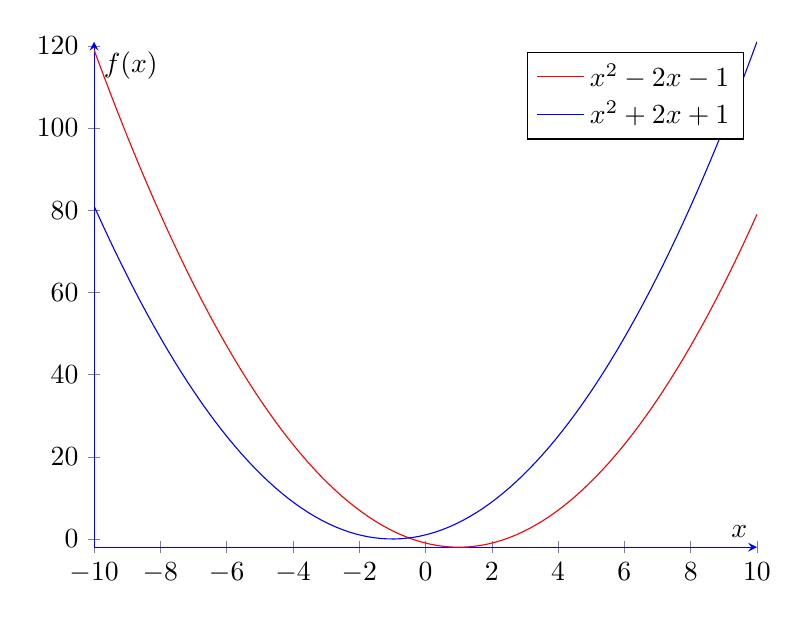
\begin{tikzpicture}
\begin{axis}[
    axis lines = left,
    xlabel = $x$,
    ylabel = {$f(x)$},
]

\addplot [
    domain=-10:10, 
    samples=100, 
    color=red,
]
{x^2 - 2*x - 1};
\addlegendentry{$x^2 - 2x - 1$}

\addplot [
    domain=-10:10, 
    samples=100, 
    color=blue,
    ]
    {x^2 + 2*x + 1};
\addlegendentry{$x^2 + 2x + 1$}
 
\end{axis}
\end{tikzpicture}
\end{document}
\end{verbatim}
\end{frame}
%matematicki
\begin{frame}
\frametitle{Primjer matematičkog grafikona}


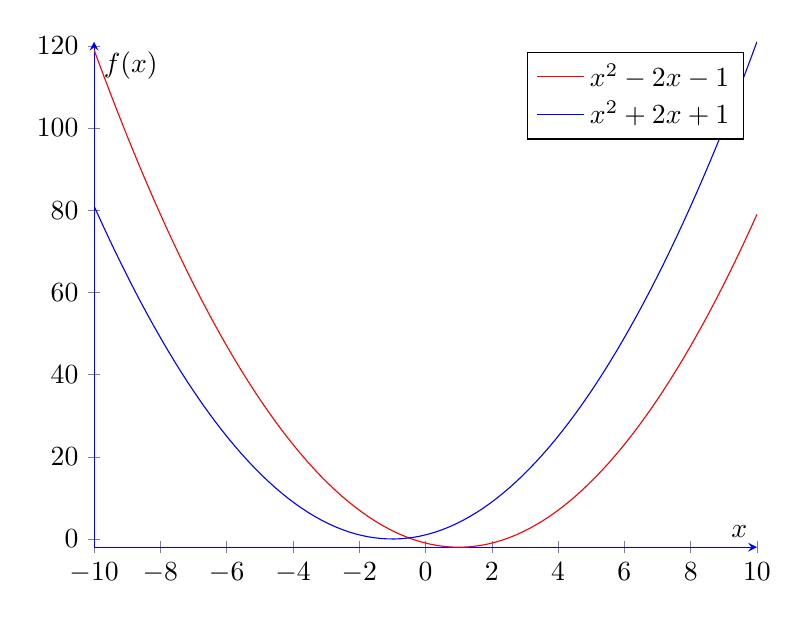
\begin{tikzpicture}
\begin{axis}[
    axis lines = left,
    xlabel = $x$,
    ylabel = {$f(x)$},
]

\addplot [
    domain=-10:10, 
    samples=100, 
    color=red,
]
{x^2 - 2*x - 1};
\addlegendentry{$x^2 - 2x - 1$}

\addplot [
    domain=-10:10, 
    samples=100, 
    color=blue,
    ]
    {x^2 + 2*x + 1};
\addlegendentry{$x^2 + 2x + 1$}
 
\end{axis}
\end{tikzpicture}


\end{frame}
%temperatura

\begin{frame}[fragile]
\frametitle{Primjer 2D grafikona}
\Fontvi

\begin{verbatim}
\documentclass[10pt]{article}
\usepackage{pgfplots}
\pgfplotsset{width=10cm,height=10cm} %dimenzije grafa
\begin{document}
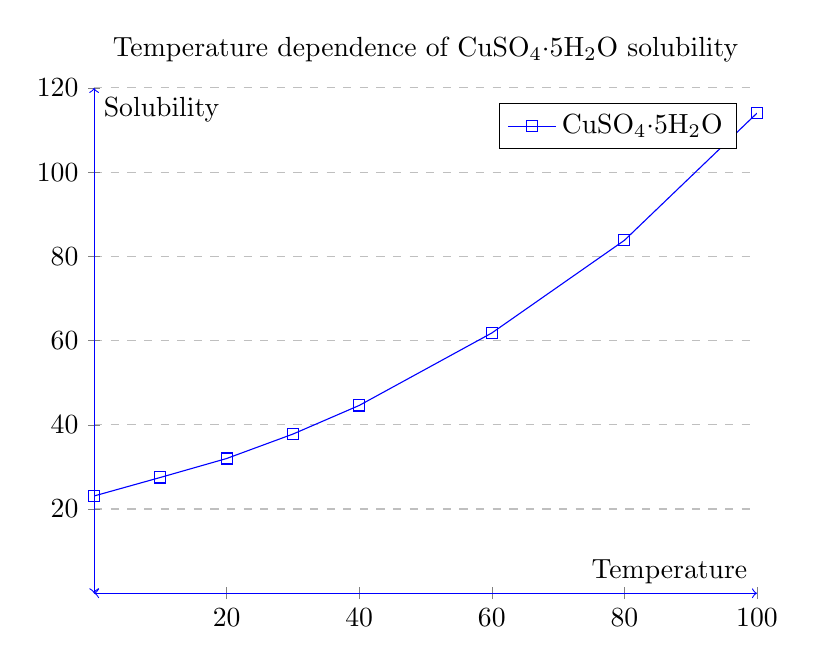
\begin{tikzpicture}
\begin{axis}[
    title={Temperature dependence of CuSO$_4\cdot$5H$_2$O solubility},
    xlabel={Temperature},
    ylabel={Solubility},
    xmin=0, xmax=100,
    ymin=0, ymax=120,
    xtick={0,20,40,60,80,100},
    ytick={0,20,40,60,80,100,120},
    legend pos=north east,
    ymajorgrids=true,
    grid style=dashed,
]
 \addplot[
    color=blue,
    mark=square,
    ]
    coordinates {
    (0,23.1)(10,27.5)(20,32)(30,37.8)(40,44.6)(60,61.8)(80,83.8)(100,114)
    };
    \legend{CuSO$_4\cdot$5H$_2$O}
 
\end{axis}
\end{tikzpicture}
\end{document}
\end{verbatim}

\end{frame}
%temperatura
\begin{frame}
\frametitle{Primjer 2D grafikona}


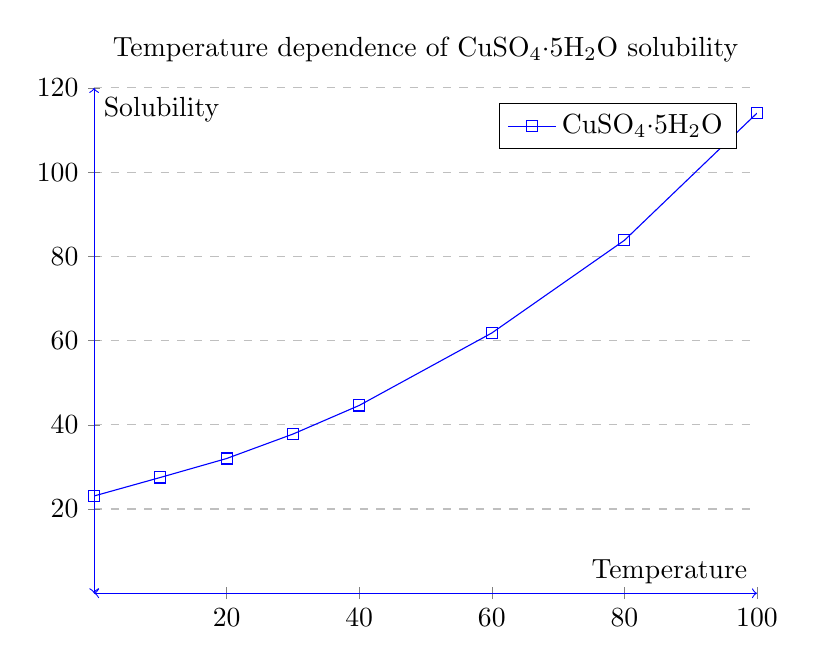
\begin{tikzpicture}
\begin{axis}[
    title={Temperature dependence of CuSO$_4\cdot$5H$_2$O solubility},
    xlabel={Temperature},
    ylabel={Solubility},
    xmin=0, xmax=100,
    ymin=0, ymax=120,
    xtick={0,20,40,60,80,100},
    ytick={0,20,40,60,80,100,120},
    legend pos=north east,
    ymajorgrids=true,
    grid style=dashed,
]
 
\addplot[
    color=blue,
    mark=square,
    ]
    coordinates {
    (0,23.1)(10,27.5)(20,32)(30,37.8)(40,44.6)(60,61.8)(80,83.8)(100,114)
    };
    \legend{CuSO$_4\cdot$5H$_2$O}
 
\end{axis}
\end{tikzpicture}


\end{frame}
%scatter grafikoni
\begin{frame}[fragile]
\frametitle{``Scatter'' grafikoni}
\textbf{Scatter} grafikoni se koriste za prikazivanje nekih informacija kao neku vrstu oznake.
Npr. prilikom računanja statističke regresije.


\end{frame}
%grafion sa stupcima
\begin{frame}
\frametitle{Grafikoni sa stupcima}

\textbf{Grafikoni sa stupcima} koriste se za prikaz prikupljenih podataka i to uglavnom statističkih podataka o nečemu.
\end{frame}
%kod grafikon sa stupcima
\begin{frame}[fragile]
\frametitle{Primjer grifikona sa stupcima}
\Fontvi

\begin{verbatim}
\documentclass[10pt]{article}
\usepackage{pgfplots}
\pgfplotsset{width=10cm,height=10cm} %dimenzije grafa
\begin{document}
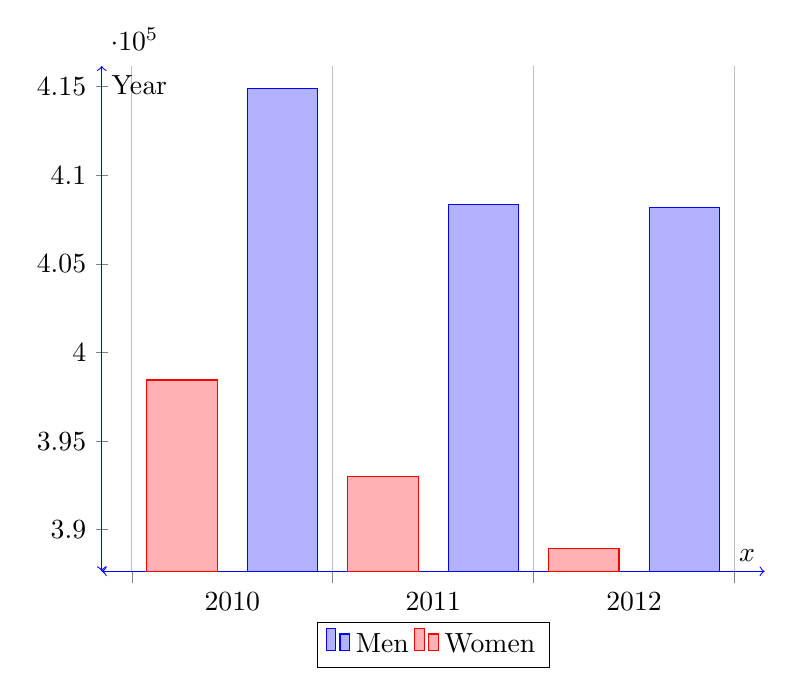
\begin{tikzpicture}
\begin{axis}[
    x tick label style={
        /pgf/number format/1000 sep=},
    ylabel=Year,
    enlargelimits=0.05,
    legend style={at={(0.5,-0.1)},
    anchor=north,legend columns=-1},
    ybar interval=0.7,
]
\addplot 
    coordinates {(2012,408184) (2011,408348)
         (2010,414870) (2009,412156)};
\addplot 
    coordinates {(2012,388950) (2011,393007) 
        (2010,398449) (2009,395972)};
\legend{Men,Women}
\end{axis}
\end{tikzpicture}


\end{document}
\end{verbatim}
\end{frame}
%grafikon sa stupcima 
\begin{frame}
\frametitle{Primjer grafikona sa stupcima}
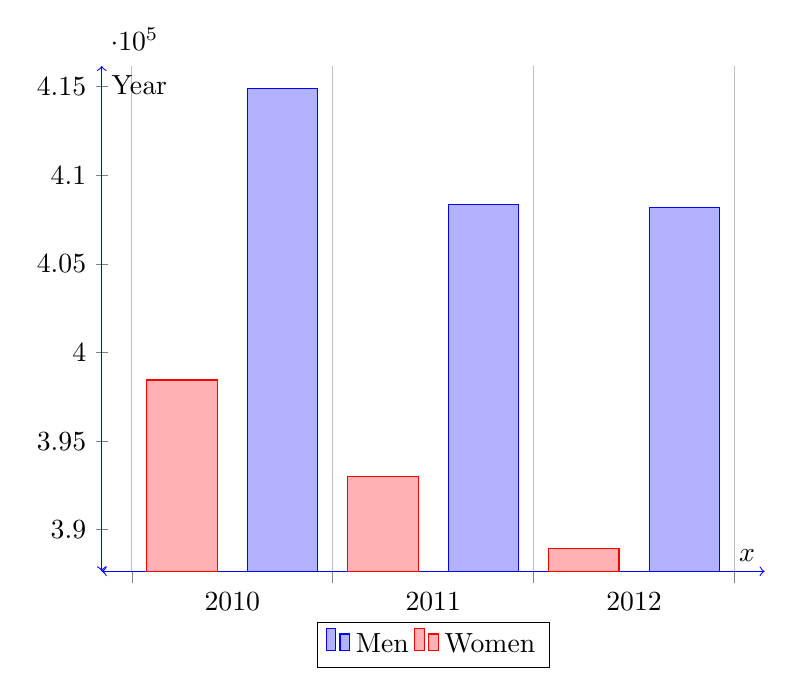
\begin{tikzpicture}
\begin{axis}[
    x tick label style={
        /pgf/number format/1000 sep=},
    ylabel=Year,
    enlargelimits=0.05,
    legend style={at={(0.5,-0.1)},
    anchor=north,legend columns=-1},
    ybar interval=0.7,
]
\addplot 
    coordinates {(2012,408184) (2011,408348)
         (2010,414870) (2009,412156)};
\addplot 
    coordinates {(2012,388950) (2011,393007) 
        (2010,398449) (2009,395972)};
\legend{Men,Women}
\end{axis}
\end{tikzpicture}
\end{frame}
%3d matematicki
\begin{frame}[fragile]
\frametitle{3D grafikon}
\Fontvi

\begin{verbatim}
\documentclass[10pt]{article}
\usepackage{pgfplots}
\pgfplotsset{width=10cm,height=10cm} %dimenzije grafa
\begin{document}
\begin{tikzpicture}
\begin{axis}[
    title=Primjer korištenja mrežnog parametra,
    hide axis, %osa se neće prikazati
    colormap/cool,
]
\addplot3[
    mesh,
    samples=50,
    domain=-8:8,
]
{sin(deg(sqrt(x^2+y^2)))/sqrt(x^2+y^2)};
\addlegendentry{$\frac{sin(r)}{r}$}
\end{axis}
\end{tikzpicture
\end{tikzpicture}
\end{tikzpicture}
\end{verbatim}
\end{frame}
\begin{frame}
\frametitle{3D grafikon}


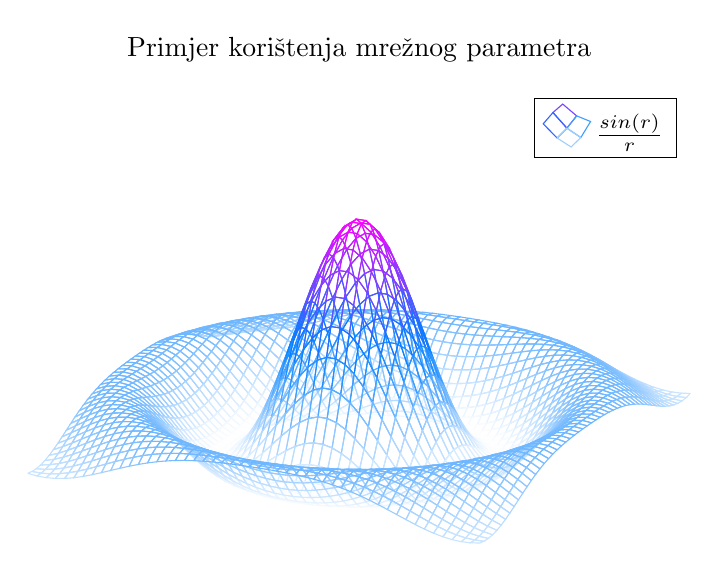
\begin{tikzpicture}
\begin{axis}[
    title=Primjer korištenja mrežnog parametra,
    hide axis,
    colormap/cool,
]
\addplot3[
    mesh,
    samples=50,
    domain=-8:8,
]
{sin(deg(sqrt(x^2+y^2)))/sqrt(x^2+y^2)};
\addlegendentry{$\frac{sin(r)}{r}$}
\end{axis}
\end{tikzpicture}

\end{frame}


\end{document}


 
 

